\documentclass[border=2pt]{standalone}
\usepackage{tikz}
\usetikzlibrary{arrows.meta,positioning,fit,calc}
\begin{document}
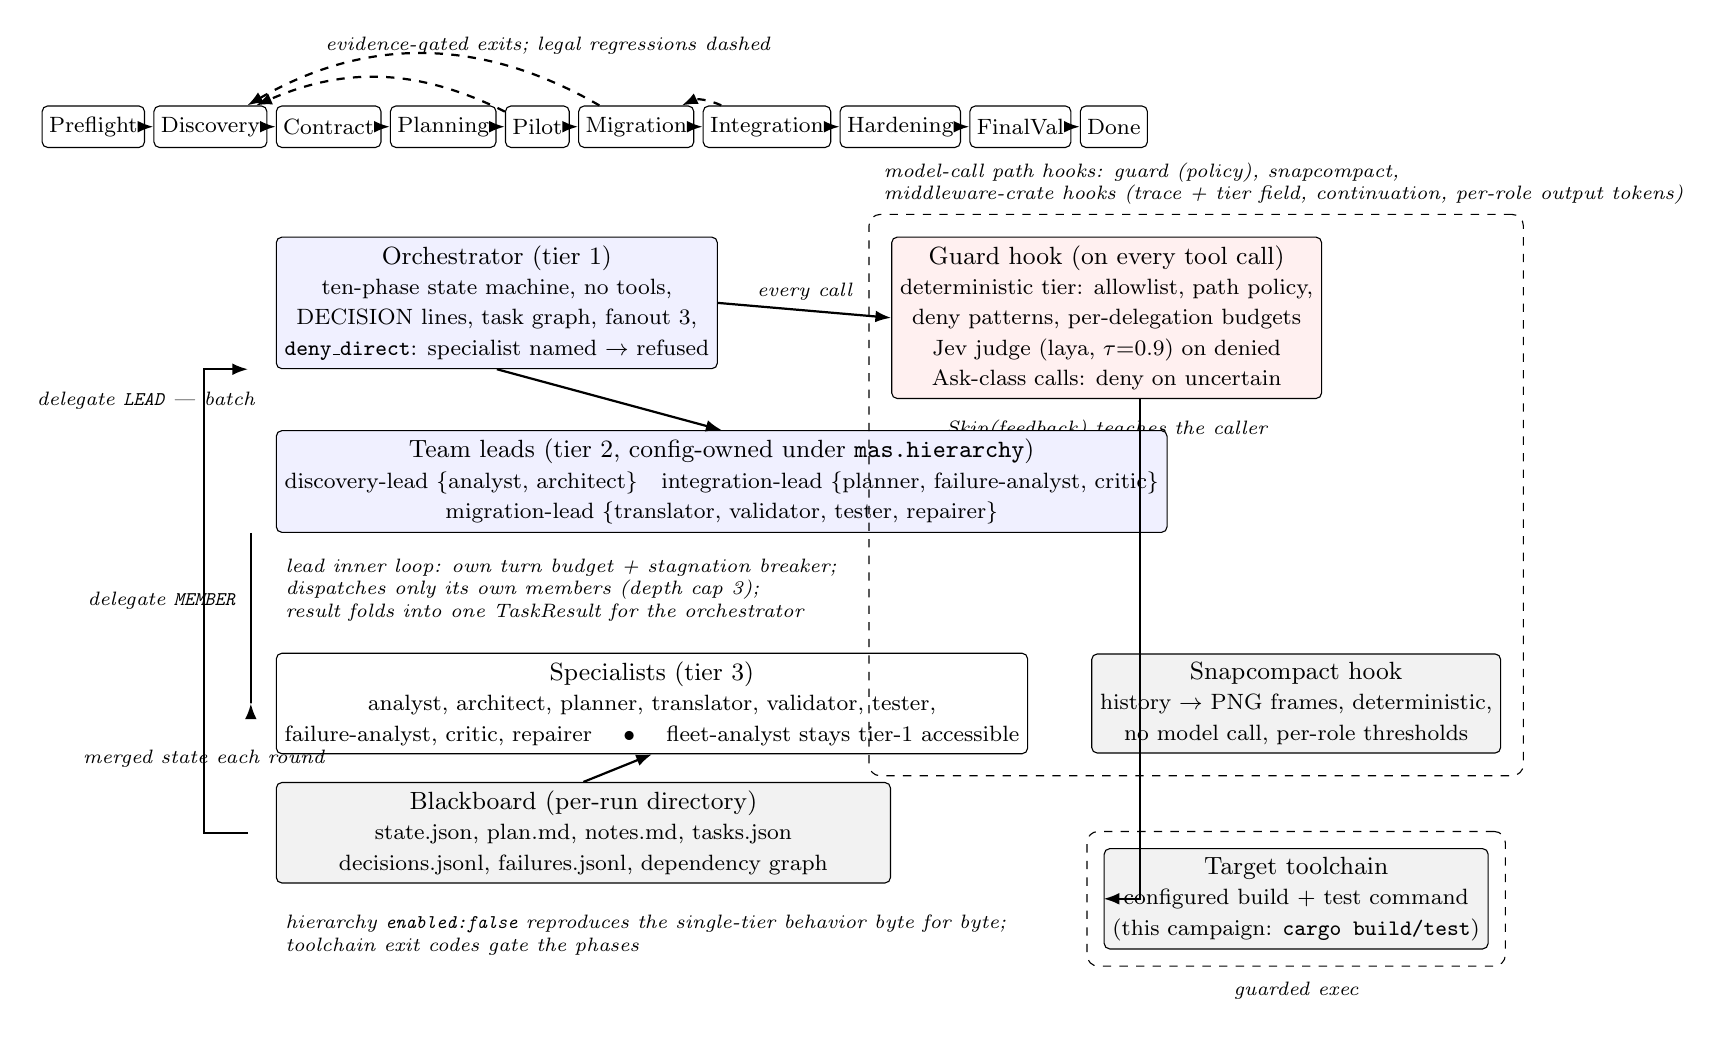
\begin{tikzpicture}[
  font=\small,
  role/.style={draw, rounded corners=2pt, align=center, inner sep=3pt, minimum height=1.5em},
  phase/.style={draw, rounded corners=2pt, align=center, inner sep=2.5pt, minimum height=1.5em, font=\footnotesize},
  arr/.style={-{Latex[length=2mm]}, thick},
  lab/.style={font=\scriptsize\itshape}
]

% ---- Phase state machine (top strip) ----
\node[phase] (p0) {Preflight};
\node[phase, right=3pt of p0] (p1) {Discovery};
\node[phase, right=3pt of p1] (p2) {Contract};
\node[phase, right=3pt of p2] (p3) {Planning};
\node[phase, right=3pt of p3] (p4) {Pilot};
\node[phase, right=3pt of p4] (p5) {Migration};
\node[phase, right=3pt of p5] (p6) {Integration};
\node[phase, right=3pt of p6] (p7) {Hardening};
\node[phase, right=3pt of p7] (p8) {FinalVal};
\node[phase, right=3pt of p8] (p9) {Done};
\foreach \i/\j in {p0/p1,p1/p2,p2/p3,p3/p4,p4/p5,p5/p6,p6/p7,p7/p8,p8/p9}
  {\draw[arr] (\i) -- (\j);}
\draw[arr, dashed] (p4) to[bend right=25] (p1);
\draw[arr, dashed] (p5) to[bend right=30] (p1);
\draw[arr, dashed] (p6) to[bend right=25] (p5);
\node[lab, anchor=south] at ($(p2.north)!0.5!(p6.north)+(0,15pt)$) {evidence-gated exits; legal regressions dashed};

% ---- Tier 1: orchestrator ----
\node[role, below=32pt of p2.south west, anchor=north west, minimum width=54mm, fill=blue!6] (orch)
  {Orchestrator (tier 1)\\ \footnotesize ten-phase state machine, no tools,\\ \footnotesize DECISION lines, task graph, fanout 3,\\ \footnotesize \texttt{deny\_direct}: specialist named $\rightarrow$ refused};

% ---- Guard hook ----
\node[role, right=22mm of orch.north east, anchor=north west, minimum width=42mm, fill=red!6] (guard)
  {Guard hook (on every tool call)\\ \footnotesize deterministic tier: allowlist, path policy,\\ \footnotesize deny patterns, per-delegation budgets\\ \footnotesize Jev judge (laya, $\tau{=}0.9$) on denied\\ \footnotesize Ask-class calls: deny on uncertain};
\draw[arr] (orch.east) -- node[lab, above]{every call} (guard.west);
\node[lab, below=4pt of guard.south] {Skip(feedback) teaches the caller};

% ---- Tier 2: team leads ----
\node[role, below=22pt of orch.south west, anchor=north west, minimum width=78mm, fill=blue!6] (leads)
  {Team leads (tier 2, config-owned under \texttt{mas.hierarchy})\\ \footnotesize discovery-lead \{analyst, architect\}\quad integration-lead \{planner, failure-analyst, critic\}\\ \footnotesize migration-lead \{translator, validator, tester, repairer\}};
\draw[arr] (orch.south) -- (leads.north);
\node[lab, anchor=south east] at ([xshift=-4pt, yshift=4pt]leads.north west) {delegate \texttt{LEAD} | batch};

% ---- Lead inner-loop note (clear of boxes) ----
\node[lab, below=6pt of leads.south west, anchor=north west, align=left] (loopnote)
  {lead inner loop: own turn budget + stagnation breaker;\\
   dispatches only its own members (depth cap 3);\\
   result folds into one TaskResult for the orchestrator};

% ---- Tier 3: specialists ----
\node[role, below=8pt of loopnote.south west, anchor=north west, minimum width=78mm] (spec)
  {Specialists (tier 3)\\ \footnotesize analyst, architect, planner, translator, validator, tester,\\ \footnotesize failure-analyst, critic, repairer \quad $\bullet$ \quad fleet-analyst stays tier-1 accessible};
\draw[arr] ([xshift=-9pt]leads.south west) |- node[lab, pos=0.2, left=2pt]{delegate \texttt{MEMBER}} ([xshift=-9pt]spec.west);

% ---- Snapcompact hook ----
\node[role, right=8mm of spec.east, anchor=west, minimum width=36mm, fill=gray!10] (snap)
  {Snapcompact hook\\ \footnotesize history $\rightarrow$ PNG frames, deterministic,\\ \footnotesize no model call, per-role thresholds};

% ---- Target toolchain ----
\node[role, below=12mm of snap.south, anchor=north, minimum width=36mm, fill=gray!10] (tool)
  {Target toolchain\\ \footnotesize configured build + test command\\ \footnotesize (this campaign: \texttt{cargo build/test})};
\draw[arr] ([xshift=12pt]guard.south) |- (tool.west);

% ---- Blackboard ----
\node[role, below=10pt of spec.south west, anchor=north west, minimum width=78mm, fill=gray!10] (board)
  {Blackboard (per-run directory)\\ \footnotesize state.json, plan.md, notes.md, tasks.json\\ \footnotesize decisions.jsonl, failures.jsonl, dependency graph};
\draw[arr] (board.north) -- (spec.south);
\draw[arr] ([xshift=-10pt]board.west) -- ++(-16pt,0) |- node[lab, pos=0.06, above]{merged state each round} ([xshift=-10pt]orch.south west);

% ---- Bottom note ----
\node[lab, align=left, anchor=north west] at ([yshift=-8pt]board.south west)
  {hierarchy \texttt{enabled:false} reproduces the single-tier behavior byte for byte;\\
   toolchain exit codes gate the phases};

% ---- Middleware/hook boundary ----
\node[draw, dashed, rounded corners=4pt, inner sep=8pt, fit=(guard)(snap)] (mwbox) {};
\node[draw, dashed, rounded corners=4pt, inner sep=6pt, fit=(tool)] (toolbox) {};
\node[lab, anchor=north] at ([yshift=-2pt]toolbox.south) {guarded exec};
\node[lab, anchor=south west, align=left] at ([xshift=2pt]mwbox.north west)
  {model-call path hooks: guard (policy), snapcompact,\\ middleware-crate hooks (trace + tier field, continuation, per-role output tokens)};

\end{tikzpicture}
\end{document}
